\section{A Primer on Causal Inference for Software Engineering Researchers}
\label{sec:primer}

Our review in Section~\ref{sec:background} established two facts: The causal inference toolkit has matured over a century of cross-disciplinary development into a set of principled methods for answering intervention-outcome questions, yet fewer than 2\% of SE papers employ any recognized causal inference method despite 29\% carrying an ambition to investigate intervention-outcome questions.
This section equips the reader with the conceptual and technical foundations needed to close that gap.
We cover the three pillars most relevant to empirical SE research---counterfactual reasoning and potential outcomes, graphical causal models, and design-based identification---and argue for a pragmatic synthesis suited to the field's observational data.
We do not cover causal discovery algorithms~\cite{journals/ese/HulseEM25}, machine-learning-based heterogeneous treatment effect estimation~\cite{chernozhukov2018double, athey2016recursive}, or formal verification of causal claims~\cite{halpern2016actual}; readers interested in these topics should consult the references cited and the textbooks listed in Section~\ref{sec:bg-causal-history}.

\subsection{What Does It Mean Exactly for X to Cause Y?}
\label{sec:primer-causality}

Consider a question that is highly relevant to SE research: Does adopting AI coding tools increase a project's development velocity?
At its core, this is a question about a contrast between two worlds---one in which a project adopts AI coding tools and one in which it does not---and whether development velocity differs between them.
This deceptively simple framing conceals a deep conceptual question: What does it \emph{mean} for one thing to cause another?
Two perspectives---one formal, one pragmatic---provide the conceptual foundation for the toolkit introduced in this section.\footnote{The philosophical literature offers additional accounts.
The most intuitive, dating to \citet{hume1748enquiry}, holds that $X$ causes $Y$ if $X$ is regularly followed by $Y$---but regular association cannot distinguish genuine causal effects from systematic differences between compared groups (Section~\ref{sec:primer-naive} makes this failure concrete).
A complementary perspective, developed by \citet{woodward2003making} and formalized through \citeauthor{pearl2009causality}'s~\cite{pearl2009causality} \emph{do-calculus}, defines causation through \emph{intervention}: $X$ causes $Y$ if intervening on $X$---holding everything else fixed---changes $Y$.
This interventionist view underpins the graphical causal model framework (Section~\ref{sec:primer-dags}), and its central insight---the difference between \emph{seeing} and \emph{doing}---recurs throughout this primer.}

\paragraph{Causation as Counterfactual Dependence.}
The formal foundation of modern causal inference, developed by \citet{rubin1974estimating} building on philosophical work by \citet{lewis1973causation}, defines causation through \emph{counterfactuals}: $X$ causes $Y$ if $Y$ would not have occurred (or would have differed) had $X$ not occurred.
Applied to our example: AI tools \emph{caused} the velocity increase for a given project if that project \emph{would have had lower development velocity} had it not adopted AI tools, all else being equal.
This definition is precise but introduces what \citet{holland1986statistics} called the \emph{fundamental problem of causal inference}: We can never observe both worlds for the same unit.
We observe the project's development velocity after adopting AI tools, or its velocity without AI tools, but never both.
The entire apparatus of causal inference---from randomized experiments to quasi-experimental designs---exists to overcome this fundamental observational limitation.
Still, the counterfactual view is useful in that it helps the researcher derive \emph{estimands}---precise definitions of the causal quantities we seek to estimate---and is formalized through the potential outcomes framework (Section~\ref{sec:primer-po}).

\paragraph{Causation as a Target Trial.}
For applied researchers, \citeauthor{hernan2020causal}'s~\cite{hernan2020causal} \emph{target trial} framework offers a pragmatic operationalization of counterfactual reasoning: Every causal question implicitly describes a hypothetical randomized experiment.
The framework asks the researcher to specify the trial they would \emph{ideally} run---the treatment, the population, the outcome, the timing, and the assignment mechanism---and then evaluate how far their observational analysis departs from this ideal.
For the AI coding tools question, the target trial would randomly assign half of a set of comparable software projects to adopt AI coding tools and compare monthly commits after a fixed period.
Articulating this trial immediately clarifies the research design and reveals threats to validity: We cannot randomly assign tool adoption, teams willing to adopt AI tools likely differ from those that do not, the ``treatment'' is ambiguous (which tools? how deeply integrated?), and commit counts may reflect development practices rather than genuine development velocity.
Each of these concerns maps directly to a specific identification assumption that must be addressed.
The target trial view also forces the researcher to confront the difference between \emph{observing} that AI-adopting projects have more commits ($P(Y \mid X\!=\!1)$) and \emph{intervening} to make a project adopt AI tools and measuring the result ($P(Y \mid do(X\!=\!1))$)---a distinction that all causal inference methods, in some sense, seek to resolve.

These two perspectives are complementary: The counterfactual view defines the \emph{target}---the causal quantity we seek to estimate---while the target trial view provides the \emph{research design template}---a concrete protocol for evaluating whether a study can credibly estimate it.
Together, they form the conceptual backbone of the three technical pillars introduced in Section~\ref{sec:primer-toolkit}: Potential outcomes formalize the counterfactual view (Section~\ref{sec:primer-po}), DAGs encode the causal structure that connects the researcher's assumptions to identification (Section~\ref{sec:primer-dags}), and design-based identification operationalizes the target trial view by exploiting quasi-random variation in the observational setting (Section~\ref{sec:primer-design}).

\subsection{Why Cannot We Use Descriptive and Correlational Evidence?}
\label{sec:primer-naive}

Before introducing the toolkit, we must understand why the approaches dominant in SE research fail to convincingly establish causation.
Two common strategies---comparing outcomes across groups and adding regression controls---each fall short in ways that motivate the formal machinery in Sections~\ref{sec:primer-toolkit}.

Consider the AI tools question again: Suppose a researcher compares monthly commits in a group of projects that adopted AI coding tools against a group of projects that did not and finds that AI-adopting projects have more commits.
Can this comparison support the claim that AI tools \emph{cause} higher development velocity?
Almost certainly not, because the two groups were never comparable to begin with.
It is very likely that projects that adopt AI coding tools differ systematically from those that do not---they may be using more AI-friendly programming languages (e.g., TypeScript and Python), have more active maintainers, more community attention, more disciplined development practices, and may belong to organizations that invest more in developer productivity.
These characteristics are \emph{confounders}: They influence both the decision to adopt AI tools (the treatment) and development velocity (the outcome), creating an association between AI tools and higher velocity even if the tools themselves have zero causal effect.
The observed difference in commit rates is a mixture of any genuine AI tool effect and the \emph{selection bias} arising from systematic differences between the compared groups---and a simple group comparison cannot disentangle the two.

The natural response is to ``control for'' these confounders using multivariate regression---e.g., one with project age, project size, number of contributors, and other covariates---and interpret the remaining coefficient on AI tool adoption as the causal effect.
This strategy is by far the most common approach to causal questions in empirical SE research, yet it suffers from at least four distinct problems plaguing many observational studies:
\begin{itemize}[leftmargin=15pt]
    \item \emph{Unobserved Confounders.}
    Regression can only adjust for measured variables, yet many confounders that plausibly affect both AI tool adoption and development velocity---e.g., developer expertise, team culture, organizational practices, project management quality---are largely unmeasurable from repository data.
    No amount of observed controls can compensate for these missing variables, and the resulting bias can be large in either direction.\footnote{Formally, if the true causal model includes an unobserved confounder $U$, the regression coefficient on the treatment converges to $\hat{\tau} \xrightarrow{p} \tau + \gamma \cdot \text{Cov}(D, U|X) / \text{Var}(D|X)$, where $\gamma$ is the effect of $U$ on the outcome and $\text{Cov}(D, U|X)/\text{Var}(D|X)$ captures the residual association between treatment and the omitted variable after partialling out the included controls (see~\citet[Ch.~3, \S3.2.2]{angrist2009mostly} for a formal derivation and \citet{cinelli2020making} for a modern sensitivity-analysis extension).
    The bias is large whenever $U$ strongly predicts both treatment $D$ and outcome $Y$.}
    \item \emph{Collider Bias.}
    When a variable is a common \emph{effect} of both treatment and outcome, conditioning on it in a regression creates spurious associations.
    For example, if GitHub popularity (e.g., star count) is influenced by both AI tool adoption (early adopters attract attention) and development velocity (active projects gain visibility), a regression with popularity as a control can manufacture an apparent relationship between AI tools and development velocity even where none exists in the full population.\footnote{In a causal directed acyclic graph (DAG), a \emph{collider} is a variable with two or more incoming arrows (e.g., $X \to C \leftarrow Y$).
    Marginally, $X$ and $Y$ may be independent, but conditioning on $C$ ``opens'' the path between them, inducing a spurious association---an effect sometimes called Berkson's paradox~\cite{berkson1946limitations}.
    Intuitively, once we know the value of a common effect, learning about one cause provides information about the other: Among popular projects, if a project did \emph{not} benefit from AI tool adoption (and its associated visibility), it likely achieved popularity through high development velocity, creating a negative association between AI adoption and development velocity that is purely an artifact of the conditioning.
    See Section~\ref{sec:primer-dags} for more details on DAGs, \citet[Ch.~1, \S1.2.3]{pearl2009causality} for the formal $d$-separation proof, and \citet{elwert2014endogenous} for an accessible treatment with social-science examples.}
    \item \emph{Mediator Bias.}
    When a variable lies \emph{on the causal pathway} from treatment to outcome, conditioning on it in a regression blocks part of the genuine effect.
    For example, if AI coding tools increase development velocity partly by automating code review and accelerating pull request throughput, then controlling for PR throughput attenuates or eliminates the very signal the researcher seeks to detect.\footnote{Formally, if the causal structure is $X \to M \to Y$ (treatment affects outcome through mediator $M$), conditioning on $M$ removes the indirect effect and leaves only the direct effect $X \to Y$.
    When the entire effect operates through the mediator---as may be the case if AI tools' velocity benefit operates entirely through faster code generation---conditioning on $M$ makes the effect vanish entirely, even though the treatment genuinely causes the outcome.
    The researcher who targets the \emph{total} effect of $X$ on $Y$ should therefore not condition on any variable on the causal pathway.
    Similarly, see \citet[Ch.~3, \S3.3.1]{pearl2009causality} for the formal derivation via the back-door criterion and \citet{wysocki2022statistical} for a demonstration of this error in applied research.}
    \item \emph{Reverse Causality.}
    Finally, regression on cross-sectional data (i.e., data collected at a single point in time) cannot determine whether AI tools increase development velocity or whether already-high-velocity teams are the ones that adopt AI tools; no set of cross-sectional controls can distinguish these two causal directions.
    Section~\ref{sec:temporal-collapse} formalizes this problem as \emph{temporal collapse}: When a cross-sectional snapshot collapses time-indexed variables into atemporal summaries, the resulting graph is cyclic and no valid adjustment set exists.
 %   \item \emph{The Table~2 Fallacy.}
 %   \citet{westreich2013table2} identified a pervasive error in which researchers interpret \emph{all} coefficients in a regression table as though each has a valid causal interpretation.
 %   A regression may be properly specified to identify the effect of one variable (say, language choice), but the coefficients on the control variables are generally confounded by their own omitted causes; presenting them as ``effects'' of those covariates is unjustified without a separate identification argument for each.
 %   The common thread across all five problems is that without a \emph{causal model} specifying the relationships among variables, researchers cannot determine which controls help, which hurt, and which coefficients admit causal interpretation---a regression with 100 covariates is not more causally credible than one with five~\cite{wysocki2022statistical}.
\end{itemize}
Despite these concerns, multivariate regression is not inherently incapable of supporting causal claims---under specific conditions, it can be a valid identification strategy~\cite{angrist2009mostly, cunningham2021causal}.
However, determining whether those conditions hold requires the formal frameworks introduced in Section~\ref{sec:primer-toolkit}: The \emph{potential outcomes framework} (Section~\ref{sec:primer-po}) defines precisely what causal quantity the researcher seeks to estimate, and the \emph{graphical causal model} framework (Section~\ref{sec:primer-dags}) provides a principled basis---through the \emph{back-door criterion}---for determining which covariates must be included, which must be excluded, and whether the remaining assumptions are plausible.
We defer the technical details to those sections, where the formalisms make the conditions precise and where design-based alternatives (Section~\ref{sec:primer-design}) offer a path forward for the many SE settings in which the regression requirements cannot be plausibly met.

\subsection{The Causal Inference Toolkit}
\label{sec:primer-toolkit}

Applied causal inference rests on three complementary pillars, each addressing a distinct question.
\emph{Potential outcomes} answer: What do we want to estimate?
They provide a formal language for defining causal estimands---the ATE, ATT, LATE---independently of any statistical model.
\emph{Graphical causal models} answer: What must we assume about the world for our estimate to be valid?
They encode causal assumptions as directed acyclic graphs (DAGs), making every assumption visible and debatable.
\emph{Design-based identification} answers: How can we exploit features of the research setting to make those assumptions credible?
Methods such as difference-in-differences, instrumental variables, and regression discontinuity derive identification from quasi-random variation rather than from the hope that all confounders have been measured.
Modern applied researchers use all three together: Potential outcomes define the target, DAGs encode the assumed causal structure, and design-based methods provide the identification strategy.

\subsubsection{The Potential Outcomes Framework}
\label{sec:primer-po}

The potential outcomes framework~\cite{neyman1923application, rubin1974estimating} formalizes the counterfactual view of causation introduced in Section~\ref{sec:primer-causality} and operationalizes the \emph{estimand-first} principle~\cite{lundberg2021estimand}: Before choosing a statistical method, the researcher must first define the causal quantity of interest.
In this section, we formally introduce this framework in the simplest binary treatment case and highlight its mathematical power in transparently articulating the \emph{identifying assumptions} needed for the estimates to carry a causal interpretation.

\paragraph{Notation and Setup.}
In the binary treatment case, each study unit $i$ has two \emph{potential outcomes}: $Y_i(1)$ under treatment and $Y_i(0)$ without treatment.
The individual causal effect $\tau_i = Y_i(1) - Y_i(0)$ is unobservable because only one potential outcome is realized---the fundamental problem of causal inference discussed in Section~\ref{sec:primer-causality}.

\paragraph{Causal Estimands.}
To get over this problem, researchers seek to estimate \emph{population-level summaries}.
One option is the \emph{Average Treatment Effect} (ATE), $\text{ATE} = E[Y(1)] - E[Y(0)]$, which answers questions like: On average across \emph{all} projects, how much does adopting AI coding tools change development velocity?
Another option is the \emph{Average Treatment Effect on the Treated} (ATT), $\text{ATT} = E[Y(1) - Y(0) \mid D = 1]$, which answers questions like: Among projects that \emph{actually adopted} AI coding tools, how much did adoption change their development velocity?
ATE and ATT coincide only under homogeneous effects or independence of treatment assignment.
Other estimands include the \emph{Local Average Treatment Effect} (LATE) for the subpopulation affected by an instrument, and \emph{conditional average treatment effects} (CATEs), $\tau(x) = E[Y(1) - Y(0) \mid X = x]$, for subgroups defined by covariates~$X$.\footnote{The LATE theorem, which shows that instrumental variables identify the causal effect for the subpopulation of \emph{compliers}, was introduced by \citet{angrist1996identification}; see \citet[Ch.~4, \S4.4--4.5]{angrist2009mostly} for a textbook treatment.
For CATEs and effect heterogeneity more broadly, a growing literature develops machine-learning estimators: \emph{Causal forests}~\cite{athey2016recursive, wager2018estimation} adapt random forests to estimate $\tau(x)$ under conditional ignorability, and \emph{double/debiased machine learning}~\cite{chernozhukov2018double} enables flexible nuisance-function estimation while preserving valid statistical inference.
These methods extend rather than replace the identification frameworks discussed in this section: A causal forest trained on data with unmeasured confounders produces biased CATE estimates, not unbiased ones.
We therefore treat effect heterogeneity as a secondary concern downstream of identification; see \citet[Ch.~10]{huntingtonklein2021effect} for an accessible introduction and Appendix~\ref{sec:appendix-faq} for further discussion.}
Which estimand to target is a substantive decision, not a statistical one: The researcher must decide whether the question concerns the average effect across all projects (ATE), the effect on adopters (ATT), the effect on the subpopulation induced to adopt by a specific mechanism (LATE), or the heterogeneity of effects across different subgroups (CATEs).

One particular power of the potential outcomes formalism is that it allows researchers to derive the \emph{identifying assumptions} required for the study's results to have a causal interpretation.
For example, in a \emph{randomized controlled trial} (RCT), the formal identifying assumption is $(Y(1), Y(0)) \perp D$ (i.e., treatment is as-if randomly assigned), so selection bias vanishes and the naive comparison identifies the ATE\@.
A valid RCT additionally requires the \emph{Stable Unit Treatment Value Assumption} (SUTVA), i.e., no interference between units and a well-defined treatment, and \emph{full compliance}, i.e., the research units are truly following their assigned treatment status.
For the family of regression, matching, and inverse probability weighting methods (for which we jointly refer to as the \emph{selection-on-observables} family), the formal identifying assumption is \emph{conditional ignorability}---the assumption that, conditional on observed covariates $X$, treatment assignment is independent of potential outcomes: $(Y(1), Y(0)) \perp D \mid X$.
Under this assumption, plus overlap ($0 < P(D\!=\!1 \mid X\!=\!x) < 1$ for all $x$ in the support of $X$), the ATE is identified through differencing the predicted outcome based on $X$:
In practice, this assumption means that all confounders must be captured in $X$ for the regression to produce a credible causal estimate, whose plausibility can be assessed through the graphical causal framework (Section~\ref{sec:primer-dags}) and complementary sensitivity analysis.\footnote{For textbook proofs that randomization identifies the ATE and that conditional ignorability identifies the ATE via regression, see \citet[Ch.~2]{angrist2009mostly} and \citet[Chs.~2--3]{hernan2020causal}.
Several methods exist to probe whether the conditional ignorability assumption is plausible:
\emph{Rosenbaum bounds}~\cite{rosenbaum2002observational} quantify how strong an unmeasured confounder would have to be to alter the study's conclusions;
\emph{coefficient stability}~\cite{oster2019unobservable} assesses whether point estimates shift substantially as controls are added, with large shifts suggesting important omitted variables;
the \emph{E-value}~\cite{vanderweele2017sensitivity} reports the minimum strength of association an unmeasured confounder would need with both treatment and outcome to explain away an observed effect;
and the \emph{robustness value}~\cite{cinelli2020making} generalizes this logic to partial $R^2$ measures, indicating how much residual variation a confounder must explain to nullify the result.
None of these methods can \emph{prove} that all confounders are measured, but they transform the unverifiable assumption into a quantitative question---\emph{how much} confounding would be required---that reviewers and readers can evaluate against in a specific setting using their domain knowledge.}

\subsubsection{Graphical Causal Models and DAGs}
\label{sec:primer-dags}

For the selection-on-observables family of methods---regression, matching, inverse probability weighting---the potential outcomes framework defines the estimand but offers limited guidance on \emph{which} variables to condition on.
As Section~\ref{sec:primer-naive} illustrated, conditioning on the wrong variables can introduce bias rather than remove it.
\citeauthor{pearl2009causality}'s~\cite{pearl2009causality} graphical framework addresses this gap by encoding causal assumptions as \emph{directed acyclic graphs} (DAGs), formalizing the interventionist view of causation introduced in Section~\ref{sec:primer-causality}.

\paragraph{Directed Acyclic Graphs.}
A DAG encodes \emph{the researcher's beliefs about the true data-generating process} and it consists of nodes (variables) and directed edges ($\to$) representing direct causal effects.
Every arrow is a substantive claim; every absent arrow asserts no direct effect.
This transparency is the central value of DAGs for applied research: Rather than debating vaguely about ``omitted variables'' or ``lurking confounders,'' researchers can argue about specific edges.
%In the programming language debate, the unproductive back-and-forth between \citeauthor{DBLP:conf/sigsoft/RayPFD14} and \citeauthor{DBLP:journals/toplas/BergerHMVV19}~\cite{DBLP:journals/corr/abs-1911-07393, DBLP:journals/corr/abs-1911-11894} could have been channeled into a productive discussion about \emph{which edges belong in the DAG} and \emph{which confounders are unmeasured}.
As a pedagogical example (without aiming for completeness), Figure~\ref{fig:ai-dag} presents a plausible DAG for the causal question of whether adopting AI coding tools affects a project's development velocity.
In this DAG, AI Tool Adoption affects Dev.\ Velocity through two \emph{mediators}---Code Generation and Workflow Automation; Team Size, Domain, Team Skill, and Project Maturity each influence both AI Tool Adoption and Dev.\ Velocity, making them \emph{confounders}; and both AI Tool Adoption and Dev.\ Velocity influence Popularity, making Popularity a \emph{collider}.
Since we care about the AI tools--velocity question, we do not show other potential edges between displayed nodes that are not relevant to the central causal question.\footnote{The sharp reader may have already noticed the fact that the DAG presented in Figure~\ref{fig:ai-dag} is ambiguous without considering the temporal nature of software engineering data: For example, the number of stars received can be a confounder \emph{before} AI tools adoption (more popular projects both exhibit higher velocity and are more likely to adopt AI tools) and a collider \emph{after} AI tools adoption (higher-velocity and AI-enabled projects are more likely to receive more stars).
We construct the proper temporal DAG and diagnose this problem formally in Section~\ref{sec:temporal-dag}.}

\begin{figure}[t]
\centering
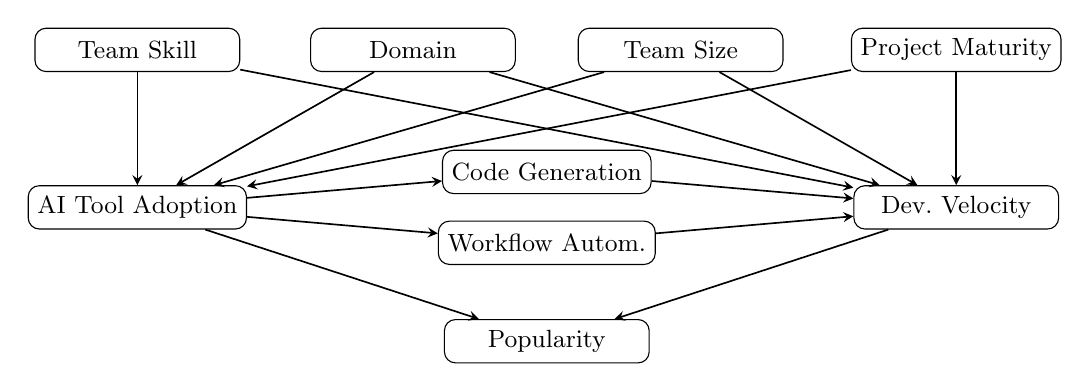
\begin{tikzpicture}[
    var/.style={draw, rounded corners, minimum width=2.6cm, minimum height=0.55cm, font=\small, align=center},
    arr/.style={->, >=stealth, semithick},
]
% Main causal chain (middle row)
\node[var] (treat) at (0, 0) {AI Tool Adoption};
\node[var] (codegen) at (5.2, 0.45) {Code Generation};
\node[var] (workflow) at (5.2, -0.45) {Workflow Autom.};
\node[var] (outcome) at (10.4, 0) {Dev.\ Velocity};
% Confounders (top row)
\node[var] (skill) at (0, 2) {Team Skill};
\node[var] (lang) at (3.5, 2) {Domain};
\node[var] (teamsize) at (6.9, 2) {Team Size};
\node[var] (maturity) at (10.4, 2) {Project Maturity};
% Collider (bottom)
\node[var] (stars) at (5.2, -1.7) {Popularity};
% Causal paths through mediators
\draw[arr] (treat) -- (codegen);
\draw[arr] (treat) -- (workflow);
\draw[arr] (codegen) -- (outcome);
\draw[arr] (workflow) -- (outcome);
% Confounders → Treatment
\draw[arr] (skill) -- (treat);
\draw[arr] (lang) -- (treat);
\draw[arr] (teamsize) -- (treat);
\draw[arr] (maturity) -- (treat);
% Confounders → Outcome
\draw[arr] (skill) -- (outcome);
\draw[arr] (lang) -- (outcome);
\draw[arr] (teamsize) -- (outcome);
\draw[arr] (maturity) -- (outcome);
% Collider paths
\draw[arr] (treat) -- (stars);
\draw[arr] (outcome) -- (stars);
\end{tikzpicture}
\caption{An example causal DAG for the AI coding tools and development velocity problem.
Arrows represent hypothesized direct causal effects.
The causal paths of interest run through two mediators: AI Tool Adoption $\to$ Code Generation/Workflow Automation $\to$ Dev.\ Velocity.
Back-door paths through common causes (e.g., AI Tool Adoption $\leftarrow$ Team Skill $\to$ Dev.\ Velocity) must be blocked for causal identification.
Popularity is a \emph{collider} (AI Tool Adoption $\to$ Popularity $\leftarrow$ Dev.\ Velocity): Conditioning on it opens a spurious path and must be avoided.}
\label{fig:ai-dag}
\end{figure}

\paragraph{Back-Door Paths and the Back-Door Criterion.}
In a DAG, \emph{causal paths} follow arrows from treatment to outcome; in Figure~\ref{fig:ai-dag}, the causal paths run AI Tool Adoption $\to$ Code Generation/Workflow Automation $\to$ Dev.\ Velocity.
These paths transmit the genuine causal effect.
A \emph{back-door path}, by contrast, connects treatment to outcome through a common cause without following the direction of the arrows---for example, AI Tool Adoption $\leftarrow$ Team Skill $\rightarrow$ Dev.\ Velocity.
These back-door paths transmit spurious associations: Even if AI tools had zero effect on Dev.\ Velocity, the fact that skilled teams both adopt AI tools earlier and inherently exhibit higher velocity creates an observed correlation between AI adoption and development velocity.
A naive comparison conflates the genuine causal effect that flows through the causal paths with the spurious associations that flow through the back-door paths.

The \emph{back-door criterion}~\cite{pearl2009causality} provides a principled rule for which variables to condition on in order to block all back-door paths without inadvertently blocking the causal paths.
A set $Z$ satisfies the criterion if (1)~no variable in $Z$ is a descendant of the treatment, and (2)~conditioning on $Z$ blocks every back-door path.
In Figure~\ref{fig:ai-dag}, $Z = \{\text{Team Size},\, \text{Domain},\, \text{Team Skill},\, \text{Project Maturity}\}$ satisfies this criterion: Each is a common cause of AI Tool Adoption and Dev.\ Velocity, and conditioning on all four blocks every spurious path.
Two types of variables must \emph{not} be included in $Z$.
Code Generation and Workflow Automation are \emph{mediators} on the causal path: Conditioning on either blocks the very effect the researcher seeks to estimate.
Popularity is a \emph{collider}: Conditioning on it \emph{opens} a spurious path rather than closing one.
When $Z$ satisfies the back-door criterion, it provides a justifiable basis that a selection-on-observables method satisfies the conditional ignorability assumption derived from the potential outcomes framework (Section~\ref{sec:primer-po}).

%the potential outcomes are independent of treatment conditional on $Z$---the graphical counterpart to the conditional ignorability assumption from Section~\ref{sec:primer-po}.
%The two frameworks are complementary: Potential outcomes define \emph{what} to estimate; DAGs determine \emph{which} variables must be conditioned on for the estimate to be valid.

%\paragraph{Alternative Explanations as Alternative DAGs.}
%Alternative explanations correspond to alternative graph structures.
%A critic might add developer motivation as an unmeasured confounder, or remove the Language $\to$ Type Safety edge entirely.
%These disagreements are productive because each alternative DAG implies testable conditional independence relations.

\paragraph{Limitations of DAGs.}
Three limitations deserve mention.
First, DAGs require \emph{domain knowledge} to construct---they encode the researcher's assumptions about the data-generating process, not knowledge derived from the data itself.\footnote{Causal discovery algorithms~\cite{spirtes2001causation} attempt to learn DAG structure directly from data, but they require their own strong assumptions (faithfulness, causal sufficiency) and remain fragile in practice.
In SE specifically, \citet{journals/ese/HulseEM25} showed that causal graph generators are unstable, with over half the discovered edges changing across minor data perturbations.
We take the stance that domain knowledge remains essential for constructing credible DAGs, though data-driven methods are an important research frontier that can complement expert judgment by suggesting edges to investigate.}
Second, a DAG's validity depends on the completeness of the variables included; omitting an important confounder renders the back-door criterion unreliable.\footnote{Sensitivity analysis tools partially address this limitation by quantifying how strong an unmeasured confounder would need to be to alter a study's conclusions---see Rosenbaum bounds~\cite{rosenbaum2002observational}, coefficient stability~\cite{oster2019unobservable}, and the robustness value~\cite{cinelli2020making}, discussed in detail in Section~\ref{sec:primer-po}.}
Third, DAGs encode qualitative causal structure (which variables affect which) but say nothing about the \emph{magnitude} or functional form of effects.\footnote{Pearl's broader structural causal model (SCM) framework~\cite{pearl2009causality} augments the qualitative DAG with functional equations and derives nonparametric identification formulas via the do-calculus.
Semiparametric estimators such as double/debiased machine learning~\cite{chernozhukov2018double} can then estimate these quantities without imposing strong functional form assumptions, bridging the gap between qualitative causal structure and quantitative effect estimation.}
Despite these limitations, DAGs remain the most practical tool for making causal assumptions transparent and debatable~\cite{rohrer2018thinking, tennant2021dags}.
For selection-on-observables methods, DAGs are indispensable: The back-door criterion provides the only principled basis for deciding which covariates to include and which to exclude.
When identification instead derives from features of the research design (Section~\ref{sec:primer-design}), DAGs play a supporting but still valuable role---providing a transparent ground for clarifying which confounders the design absorbs and which still remain as potential threats.

\subsubsection{Design-Based Identification}
\label{sec:primer-design}

The preceding section showed how DAGs guide covariate selection for regression and matching---methods that identify causal effects under the assumption that \emph{all} confounders are observed and adjusted for.
In many SE settings, where key confounders such as developer skill, team culture, and organizational practices are largely unmeasurable from repository data, justifying this assumption is challenging.
\emph{Design-based identification} takes a fundamentally different approach: Rather than attempting to measure and adjust for all confounders, it exploits features of the research setting---temporal variation, natural experiments, assignment thresholds---that provide quasi-random variation in treatment assignment.
This essentially creates a \emph{natural experiment} setting that would approximate the ideal target trial~\cite{dunning2012natural,hernan2020causal}.
The credibility of these methods derives not from the completeness of the causal theory but from the transparency and partial testability of their design-specific assumptions~\cite{angrist2010credibility}.

\begin{table}[t]
\centering
\caption{Common causal inference methods, their target estimands, and key identification assumptions under the potential outcomes framework.
ATE = Average Treatment Effect; ATT = Average Treatment Effect on the Treated; LATE = Local Average Treatment Effect.
We use precise terminologies in this table; see the references for detailed explanations of these terminologies.}
\label{tab:methods-summary}
\footnotesize
\begin{tabular}{@{} p{3.2cm} p{1.6cm} p{8.2cm} @{}}
\toprule
\textbf{Method} & \textbf{Estimand} & \textbf{Key Identification Assumptions} \\
\midrule
Randomized Controlled Trial
  & ATE
  & Random assignment: $(Y(1), Y(0)) \perp D$; SUTVA; full compliance \cite[Ch.~4]{cunningham2021causal} \\
\addlinespace
Selection on Observables {\scriptsize (Regression, Matching, IPW)}
  & ATE / ATT
  & Conditional ignorability: $(Y(1), Y(0)) \perp D \mid X$; overlap; correct functional form for parametric estimators \cite[Ch.~3]{angrist2009mostly}, \cite[Ch.~5]{cunningham2021causal} \\
\addlinespace
Difference-in-Differences
  & ATT
  & Parallel trends: absent treatment, treated and control groups would have followed the same trajectory; no anticipation; SUTVA \cite[Ch.~5]{angrist2009mostly}, \cite[Ch.~9]{cunningham2021causal} \\
\addlinespace
Instrumental Variables
  & LATE
  & Relevance: instrument $Z$ affects treatment; exclusion: $Z$ affects outcome only through treatment; independence; monotonicity (no defiers) \cite[Ch.~4]{angrist2009mostly}, \cite[Ch.~7]{cunningham2021causal} \\
\addlinespace
Regression Discontinuity
  & LATE \scriptsize{(at cutoff)}
  & Continuity of potential outcomes at threshold; no precise manipulation of running variable; no compound treatments at cutoff \cite[Ch.~6]{angrist2009mostly}, \cite[Ch.~6]{cunningham2021causal} \\
\addlinespace
Panel Fixed Effects
  & ATE \scriptsize{(within-unit)}
  & Strict exogeneity: conditional on unit FE, treatment is uncorrelated with time-varying unobservables; no time-varying confounders \cite[Ch.~5]{angrist2009mostly}, \cite[Ch.~8]{cunningham2021causal} \\
%\addlinespace
%Synthetic Control
%  & ATT \scriptsize{(treated unit)}
%  & Synthetic control tracks treated unit's counterfactual trajectory; no interference; no anticipation \\
\bottomrule
\end{tabular}
\end{table}

Table~\ref{tab:methods-summary} summarizes the methods most relevant to SE research, along with their formal estimand and identifying assumptions derived from the potential outcomes framework (see \citet[Chs.~2--6]{angrist2009mostly} and \citet[Chs.~4--9]{cunningham2021causal} for formal proofs and detailed treatments of each method).
In this section, we illustrate the high-level idea of each method with SE examples to build intuition:

\begin{itemize}[leftmargin=15pt]
    \item \emph{Difference-in-Differences (DiD).}
    DiD compares changes in outcomes over time between a treated group and a control group, e.g., comparing development velocity trends before and after AI tool adoption in treatment repositories versus comparable repositories that did not adopt.
    The key assumption---\emph{parallel trends}---requires that, absent the adoption, both groups would have followed the same outcome trajectory.
    This assumption can be partially assessed using pre-treatment trend tests, and modern estimators leverage staggered adoption to construct natural experiments among treated units with different adoption timings~\cite {callaway2021difference, roth2023whats}.
    The DiD methodology has been successfully applied in SE settings to study the impact of social media promotion on open-source project popularity and contributor attraction~\cite{DBLP:conf/icse/FangLHV22}, the impact of core contributor disengagement on open-source project workflows~\cite{DBLP:conf/icse/ChenSSGT26}, and the impact of Cursor adoption on development velocity and code quality~\cite{DBLP:conf/msr/HeMAKV26}.
    As a tutorial example, we will apply staggered DiD to the AI coding tools question in Section~\ref{sec:did}.

    \item \emph{Instrumental Variables (IV).}
    IV uses an \emph{instrument}---a variable that affects the treatment but influences the outcome only through the treatment---to isolate exogenous variation.
    The IV estimand is the LATE---the effect on units whose treatment status was changed by the instrument~\cite{angrist1996identification}.
    \citet{DBLP:journals/tosem/GrafVlachyW24} provide a comprehensive tutorial on applying IV and two-stage estimation in SE research, using the observed correlation between indentation style (tabs vs. spaces) and developer salary---where programming language acts as an omitted confounder---to illustrate how IV can recover consistent causal estimates when conventional regression is biased by endogeneity.

    \item \emph{Regression Discontinuity (RDD).}
    RDD exploits \emph{sharp} thresholds in treatment assignment to create a quasi-experimental contrast in the outcome between units just above and just below the threshold.
    For example, if open-source projects exceeding a certain popularity threshold are eligible for a sponsorship program, comparing projects just above and just below the threshold provides a quasi-experimental contrast in the program's outcomes.
    Identification requires that potential outcomes are continuous at the threshold and that units cannot precisely manipulate their position relative to the cutoff.
    To our knowledge, we are unaware of a successful RDD application in an SE setting (see previous footnote in Section~\ref{sec:bg-adoption} for a discussion of terminology misuses).

    \item \emph{Panel Fixed Effects.}
    Panel fixed effects models compare repeated observations of the same unit over time, absorbing all \emph{time-invariant} characteristics through unit-specific intercepts.
    For example, observing the same repository before and after AI tool adoption removes confounding from all time-invariant repository characteristics---codebase domain, long-term team composition, organizational practices---that cross-sectional comparisons cannot address.
    The identifying assumption is \emph{strict exogeneity}: Conditional on unit fixed effects, the treatment is uncorrelated with time-varying unobservables (i.e., no time-varying confounders that are left unmeasured).\footnote{This assumption differs from the conditional ignorability assumption from selection-on-observables methods: Panel fixed effects automatically absorb all time-invariant confounders without requiring them to be measured, but the researcher must still argue---using domain knowledge or a DAG---that no unmeasured time-varying confounders remain and that past outcomes do not feed back into future treatment assignment.}
    Panel fixed effects models have been applied in SE settings to study the causal impact of code quality on developer productivity at Google~\cite{DBLP:conf/sigsoft/ChengMCJGKZ022}.
    They are also often used as a baseline model for DiD designs (see Section~\ref{sec:did} for an example).

%    \item \emph{Synthetic Control.}
%    Synthetic control constructs a weighted combination of untreated units to serve as a counterfactual for a single treated unit.
%    In SE: To estimate the effect of a major framework's migration to TypeScript, one could construct a ``synthetic'' control from similar frameworks that did not migrate, weighted to match the treated framework's pre-migration defect trajectory.
\end{itemize}

\subsection{A Pragmatic Stance for Software Engineering Research}
\label{sec:primer-stance}
\label{sec:guide}

The preceding subsections introduced a rich but potentially daunting toolkit: Potential outcomes define estimands, DAGs encode mechanisms, and design-based methods exploit quasi-random variation.
An SE researcher encountering these ideas for the first time faces an immediate practical question: \emph{How do I actually use this?}
In general, there is no universal recipe for causal inquiries in \emph{any} research setting---causal inference requires both methodological rigor and creative problem-solving, and the ``right'' approach depends on the specific features of the data and setting.
Drawing on the emerging consensus across econometrics~\cite{imbens2020potential, angrist2010credibility}, epidemiology~\cite{hernan2020causal}, and sociology~\cite{lundberg2021estimand}, we recommend a pragmatic synthesis tailored to the realities of empirical SE research as follows.

\paragraph{Build on Prior Research and Practitioner Knowledge.}
\label{sec:stance-prior-research}
Every step of a causal inquiry---framing the question, proposing a DAG, choosing covariates---requires \emph{domain knowledge} that cannot be derived from the data alone.
In SE, this knowledge comes from three sources.
First, prior quantitative studies provide the raw material for proposing causal structures: An observed association between AI tool adoption and development velocity does not itself establish causation, but it motivates a DAG edge that can then be subjected to rigorous identification.
Second, gray literature---blog posts, postmortems, industry reports, conference talks---encodes rich practitioner causal beliefs (``we adopted X and Y improved'') that inform which mechanisms are plausible and which confounders are likely.
Third, qualitative SE research---interviews, case studies, grounded theory---surfaces causal reasoning that developers and teams use in practice, providing mechanistic accounts that purely quantitative data cannot.
These sources collectively generate the theories that causal methods then test, creating a virtuous cycle: Prior work proposes causal structures, rigorous methods evaluate them, and the findings refine theory for the next iteration.

\paragraph{Use Counterfactual Reasoning to Frame Research Designs.}
\label{sec:guide-question}
Before analyzing data, articulate the \emph{target trial}: What randomized experiment would you ideally run?
What is the treatment, the population, the outcome, and the timing?
This exercise forces clarity about aspects that SE studies often leave implicit---for example, whether ``AI tool adoption'' refers to code generation, automated review, or the broader workflow changes that accompany the tools.
The target trial framework is especially natural for SE researchers who are already familiar with controlled experiments~\cite{DBLP:books/sp/WohlinRHORW24}: It simply asks them to describe the experiment they wish they could run and then evaluate how far their observational design departs from this ideal.

\paragraph{Use DAGs to Reason About Mechanisms and Covariate Selection.}
\label{sec:guide-path-a}
Once the target trial is articulated, construct a DAG encoding the assumed causal structure.
The DAG identifies which covariates must be controlled for (back-door criterion), which must \emph{not} be controlled for (mediators and colliders), and makes every assumption explicit so that reviewers can challenge specific edges rather than raising vague concerns.
While the DAG is less central to identification for design-based methods, it remains valuable for reasoning about which confounders the design absorbs, what remaining threats exist, and more importantly, what is the actual \emph{mechanism} behind the observed cause and effect.
A genuine and rigorous reasoning on causal mechanisms often reveals important design considerations and practical implications, as we demonstrate in the worked example: The temporal DAG (Section~\ref{sec:temporal-dag}) reveals that many commonly used cross-sectional covariates are temporally ambiguous, motivating a shift from covariate adjustment to design-based identification (Section~\ref{sec:longitudinal}).

\paragraph{Use Design-Based Identification When the Setting Permits.}
\label{sec:guide-identification}
\label{sec:guide-path-b}
When the data contain temporal variation (panel data), staggered adoption events (DiD), plausible instruments (IV), or assignment thresholds (RDD), exploit these features rather than relying solely on covariate adjustment.
Table~\ref{tab:design-features} maps common data features to the appropriate design-based method with SE examples.
Different methods estimate different quantities---DiD identifies the ATT, IV recovers the LATE, RDD identifies an effect at the threshold---so the choice should be guided by the research question and available data structure, not convention.
Design-based methods are not assumption-free; they replace the untestable no-unobserved-confounders assumption with different assumptions (parallel trends, exclusion restrictions, continuity) that must be argued substantively---but these assumptions are typically more transparent and partially testable.
Every study navigates a tension between internal validity (causal confidence) and external validity (generalizability), and the pragmatic researcher chooses the strongest credible design and builds confidence through \emph{triangulation}: convergent findings across complementary designs, data sources, and populations~\cite{shadish2002experimental}.

\begin{table}[t]
\centering
\caption{Mapping data features to design-based identification strategies.}
\label{tab:design-features}
\footnotesize
\begin{tabular}{@{} p{3.8cm} p{2.2cm} p{6.5cm} @{}}
\toprule
\textbf{Data Feature} & \textbf{Method} & \textbf{SE Example} \\
\midrule
Same units observed over time & Panel FE & Developers contributing in multiple languages across projects \\
[0.3em]
Staggered adoption events & DiD & Projects adopting a linter at different times \\
[0.3em]
External shock affecting treatment & IV & Platform policy mandating a practice \\
[0.3em]
Threshold-based assignment & RDD & Eligibility for a program based on project size or popularity\\
\bottomrule
\end{tabular}
\end{table}

\paragraph{Iterate Between Question, Assumptions, and Design.}
The activities above---target trial, estimand, DAG, identification strategy---are presented sequentially but the process is iterative.
Constructing the DAG may reveal that the treatment is poorly defined, sending the researcher back to reformulate the target trial.
Defining the estimand may reveal that the question of interest (e.g., ATT vs.\ ATE) constrains which identification strategies are feasible.
Discovering a quasi-experimental feature in the data may suggest a sharper estimand than originally planned.
This iterative refinement is not a failure of planning but an integral part of rigorous causal reasoning.

\paragraph{When Clean Identification Is Unavailable.}
\label{sec:guide-neither}
Many SE settings do not neatly fit either path: For example, the DAG may reveal unmeasured confounders, the quasi-experimental variation may not control important unobserved confounders, or the treatment and outcome are not well-defined.
This is not a failure of empirical research but rather the norm; the pragmatic response is to use the best available strategy and be transparent about the limitations and the direction of likely bias.
Conclusions should be framed as ``consistent with a causal interpretation under assumptions X, Y, Z'' rather than as definitive causal claims.
The researcher should also consider whether the causal question can be \emph{reformulated} to exploit available variation---often the most creative and valuable act in a causal inquiry, transforming an intractable question into a tractable one (e.g., ``Does the adoption of certain programming language improve software quality?'' is intractable from cross-sectional data, but ``Does adopting type systems decrease defect proneness?'' can be studied with a difference-in-differences design if adoption events are observable).
An honest, well-argued correlational analysis or an imperfect design-based identification strategy that explicitly states its limitations is more valuable than a spurious claim of causation pretending that certain methods ``automatically bring causality.''
Indeed, the full disclosure of what a study \emph{cannot} identify is one of the causal framework's most powerful outputs: It converts each unfulfilled assumption into an explicit pointer toward a stronger future design---telling the next researcher precisely what data to collect, what variation to exploit, or what confounder to measure.

\paragraph{Engage with Alternative Explanations.}
\label{sec:guide-credibility}
After choosing an identification strategy, the researcher must honestly assess its fragility and engage with rival explanations.
Limitations should be \emph{mitigated}, not merely listed---as \citet{DBLP:journals/tosem/RobillardAEGLNNSSS24} argue for threats-to-validity sections generally, the causal setting demands that each limitation be engaged with substantively, not catalogued perfunctorily.
Three common patterns of alternative explanations arise in SE research.
\emph{Alternative mechanism}: The treatment effect operates through a different pathway than hypothesized; conditioning on the alternative mediator should attenuate the effect.
\emph{Unmeasured confounding}: A hidden variable drives both treatment and outcome; sensitivity analysis (Rosenbaum bounds, robustness values) quantifies the required strength, and falsification tests probe whether the confounding story predicts spurious effects on unrelated outcomes.
\emph{Reverse causality}: The outcome drives the treatment rather than the reverse; panel data can reveal temporal signatures that distinguish causal direction.
SE research faces distinctive measurement challenges that compound these threats: noisy proxies for latent constructs (e.g., bug-fix commits as a proxy for defect proneness), construct validity issues (e.g., lines of code as a measure of complexity), and potential SUTVA violations in interconnected software ecosystems where one project's treatment spills over to affect another's outcomes.
The mark of a credible causal study is not the absence of limitations but the transparency and rigor with which they are addressed---and the degree to which honestly stated limitations chart a path for subsequent work to follow.

\paragraph{Promises and Perils of Causal Inference in Empirical SE}
Some features of the SE research landscape make this synthesis particularly promising.
First, SE data is inherently \emph{panel data}: Repositories have temporal structure, developers contribute over time and across projects, and tools are adopted in staggered fashion---making DiD, panel FE, and synthetic control designs natural fits.
Second, SE ecosystems generate rich quasi-experimental variation: Company policies mandate practices, projects adopt practices in staggered waves, and migrations create sharp treatment contrasts---all of which offer credible identification strategies that purely cross-sectional analysis cannot exploit.
Finally, SE's rich body of quantitative studies, qualitative investigations, and gray literature provides fertile ground for theory proposition and DAG formulation---decades of empirical findings, practitioner postmortems, and case studies supply the domain knowledge needed to propose plausible causal structures before any identification strategy is chosen.

On the other hand, several SE-specific challenges also temper these promises and require careful consideration by the SE researcher.
First, SE's observational data is plagued by unmeasured confounders---developer skill, team culture, organizational practices---that are rarely captured in repository data, making design-based identification or sensitivity analysis of unmeasured confounders essential.
Second, SE treatments are often \emph{compound}: For example, ``adopting AI coding tools''---as identified by AI configuration files in a repository---bundles the tools themselves, the workflow reorganization that accompanies systematic adoption, and the self-selection of teams willing to integrate AI into their process; the researcher should interpret the estimated effect as the effect of this entire bundle rather than attribute it to a single oversimplified treatment (e.g., ``just use AI coding tools to ship faster'').
Third, interconnected software ecosystems create \emph{SUTVA violations}: Shared libraries propagate treatment effects across projects, developer mobility carries practices between teams, and upstream changes spill over into downstream dependencies.
Careful unit definition and robustness checks can bound this threat, and recent advances in causal inference under network interference provide promising tools~\cite{savje2021average, forastiere2021identification}, but adapting these methods to SE's sociotechnical structures---where spillover propagates simultaneously through dependency graphs, developer networks, and ecosystem coupling---remains an open frontier.
Finally, SE outcomes are typically \emph{noisy proxies} for the constructs of interest: Number of commits proxy for development velocity, lines of code proxy for project complexity, and star counts proxy for popularity---each introducing measurement error that may attenuate effect estimates and complicate interpretation.
One can strengthen the evidentiary basis by triangulating across multiple outcome measures that capture different facets of the same construct~\cite{lawlor2016triangulation} and conducting measurement error analysis to bound attenuation bias~\cite{hausman2001mismeasured}.
More broadly, \emph{measurement} and \emph{identification} are orthogonal challenges: A perfectly identified design still produces misleading conclusions if the outcome proxy is invalid, and a perfectly measured outcome still conflates causal effects with confounding if the design lacks identification.
The causal inference toolkit addresses identification; measurement validity requires its own careful attention---including construct definition, proxy validation, and sensitivity to measurement error---that this tutorial acknowledges but does not attempt to resolve.
Importantly, each peril on the identification side has a principled response within the toolkit so that SE researchers can engage with the specific threats in their settings.
To faciliate constructive evaluation of SE studies with causal claims, we provide an empirical standard for causal inquiries following the format of the ACM SIGSOFT Empirical Standards (Appendix~\ref{sec:appendix-standard}).
